\section{Results and Analysis}
\label{S:5}


% \subsection{Security}

% \subsubsection{In compare with the previous GSLS}

% \begin{itemize}
%   \item Now data are sent in an encrypted way - Communication channel is secure
%   \item Data are "more distributed" not only in the GSLS network but over all the nodes
%   \item Not possible to create replication/replay attack (or whatever is called, where you basically repeat the same instruction)
%   \item Built in versioning system
%   \item Nonce problem (one node could always return a wrong nonce), change the GSLS server
% \end{itemize}

% \subsubsection{In compare with light client}
% \begin{itemize}
%   \item This is a light client, just very light, it allows only few operations (not possible to hack it with other transactions if not the one we wrote in the abi file ) <-- confirm that
%   \item All the security of a cold wallet (no 3rd party knows it), but still able to create transactions.
%   \item No need to install particular and specific blockchain nodes or to run any particular program in background. The Identity management over the Social Networks is a service widely used by the majority of the developed countries therefore must be easy to use and plug & play. [in our case you register as if a normal website -> with the same complexity for the user]
% \end{itemize}


What we can infer from the proposed implementation is that GSLS becomes an Ethereum node which proxies the user requests to the Ethereum node itself. The users must download a desktop application (or can build the transaction by themselves). It is recommended that this process is carried out off-line in order to avoid hijacking attack.

\subsection{Write operation}

The writing requests were divided based on the \textit{gasPrice} measured in gigawei (GWei). The requests run using the suggested \textit{gasPrice} (30 GWei) were executed 17 seconds on average, with 9.8 seconds minimum and 47 seconds maximum. These figures are much higher than 2.312, the average writing time of the current GSLS version \cite{gondor_distributed_2016}. The reason for such a long time depends on both the workflow and the mining time. 
% The user must create or own a \textit{key pair} (public \& private key) on the client side (See Electron desktop application in the appendix).
In order to create a new transaction, the sender must know her \textit{nonce}, the current \textit{gasPrice} and the \textit{gasLimit}. This values are available to any node, therefore the desktop application sends a GET request to the GSLS along with its account address. Once all the fields are known to the sender, she creates an off-line transaction and signs is with her private key, encodes it via RLP and sends to the GSLS server. The first GET request is usually sent only at startup time and, therefore, has been omitted in the write request time calculation. 

Once the GSLS server receives the transaction it can optionally verify the content of the transaction (finding the public key of the sender via elliptic curve recovery) or directly forward the transaction to Ethereum node. The transaction will there be analysed and ran in the EVM. If correct, it is validated, mined and broadcasted to the network.

\begin{figure}[h]
	\centering
  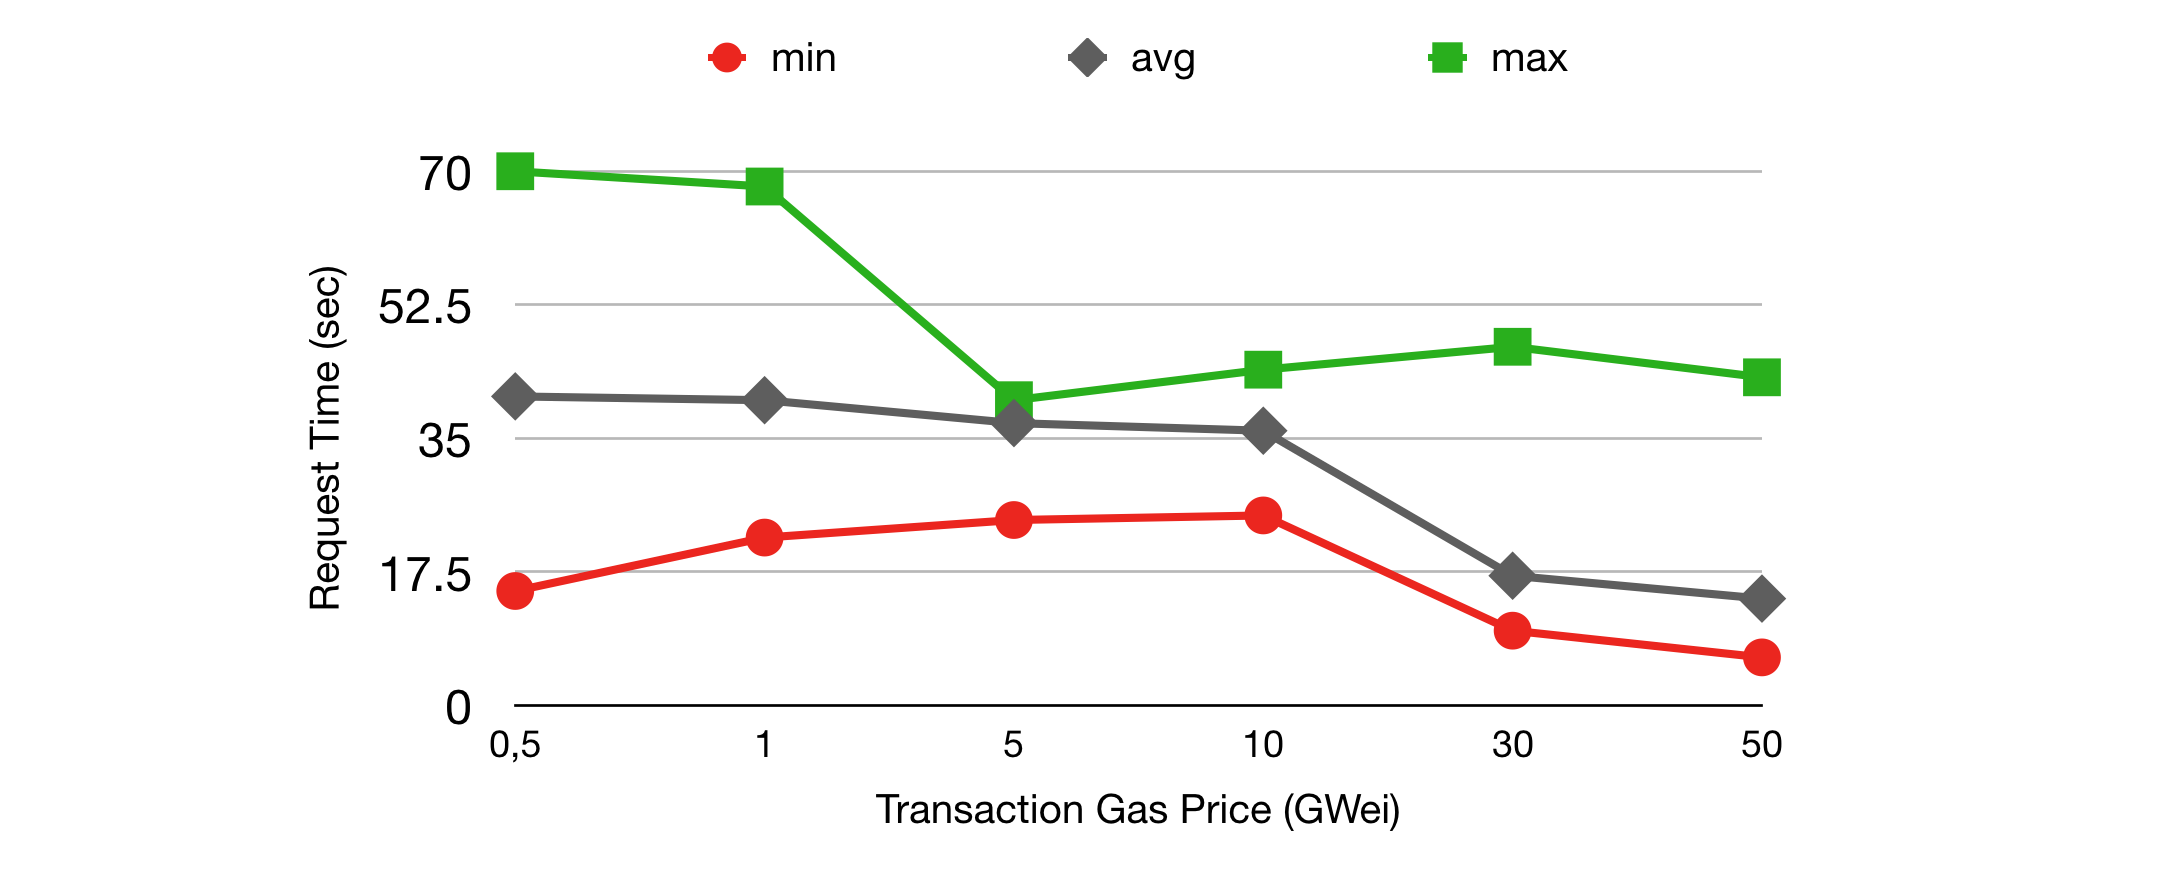
\includegraphics[width=1\textwidth]{write}
	\caption{Minimum, maximum and average time for the write operation.}
	\label{fig4}
\end{figure}

The plot shows how the reading time is bound to the blockchain mining and how it is possible to decrease the mining time by setting higher \textit{gasPrices}. This depends on the fact that higher gas prices increase the chance of a transaction to be included in the next block. Therefore, the average writing time can't be lower than a single block mining time. This value is 15 seconds on average\footnote{For more information, visit https://ethstats.net/}. 

\subsection{Read operation}

The analysis of the log file showed that the average time for request to be completed was of 1.120 seconds, while the median time was 0.968 seconds. The results showed also that 75\% of the requests were executed in less than 1.062 seconds. We can see that the average time is one order of magnitude higher compared to the previous implementation (average response time of 0.034 seconds \cite{gondor_distributed_2016}). 

These results heavily depend on the decision to use an on-line blockchain service. In fact, the GLSL needs to make an additional HTTP request, thereby adding more delay. In the ideal case, the GSLS node hosts the blockchain and the reading time is almost negligible.

In fact, a digital resource or a physical user that wants to access a SR given its associated \textit{globalId} can retrieve this information from the blockchain via a contract \textit{call} (or a \textit{message call}, if two contracts are exchanging information). This call can be done locally by any node in the network as the information is replicated and publicly available, thus Ethereum distinguishes it using the keyword \textit{constant} which means that the execution of such instruction does not change the state in the blockchain.
In other words the situation described in \ref{ethereumEcosystem:1} $t(\sigma_t) = \sigma_{t+1}$ is such as $\sigma_t = \sigma_{t+1}$ and therefore the specific transaction $t$ can be ignored by the distributed system and be run locally without any gas cost.

Since the read operations do not change the state (i.e. do not require a transaction) they are free. Furthermore, in case the user is hosting the blockchain, the operation is also fast since the information is locally available.

As an example, given a social network A, it can retrieve the SR related to the user X in another social network B, then make an HTTP call to social network B asking for a particular event and finally report the information to user X. It is possible to notice that the user X does not need to be registered in the social network B.

\begin{figure}[h]
	\centering
  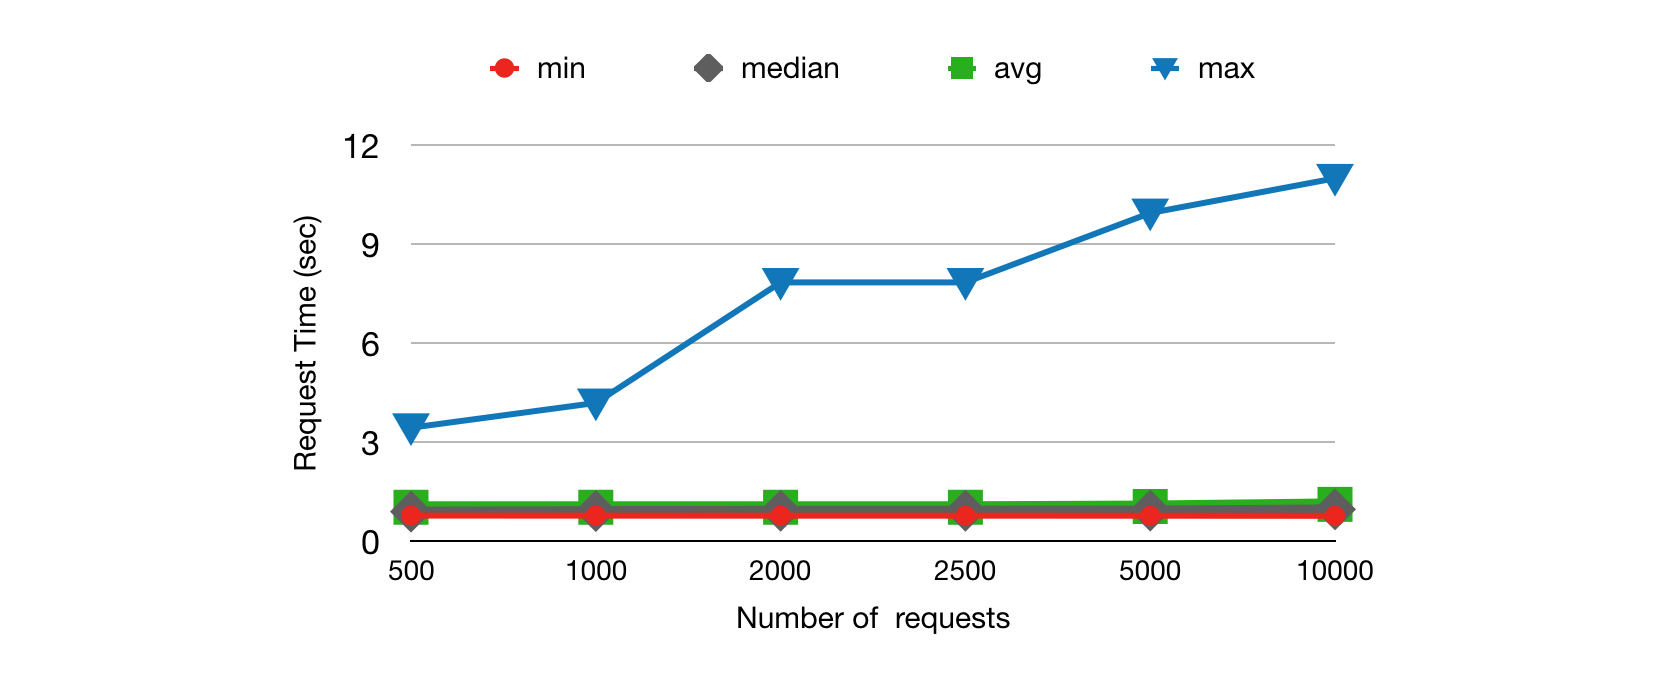
\includegraphics[width=1\textwidth]{read}
	\caption{Minimum, maximum, average and median time for the read operation.}
	\label{fig4}
\end{figure}

We can consider this results as representing the \textit{user perspective} on the read request (i.e. the time  of the HTTP request plus the execution and HTTP response). The tests run on the previous GSLS version considered only the execution time and not the the HTTP request and response time. Therefore, we can infer that the reading times in the two versions are similar in case we use this user perspective (and the GSLS node hosts a blockchain node).

% \subsection{Solidity data structures}
% Solidity is the name of the Ethereum contract language. It is designed to optimize the efficiency and memory of the EVM and, for these reasons, it does not allow arrays with undefined length.
% Therefore we map types in a key-value fashion.

% One data structure is requires to map the sender's address with its own \textit{globalId} (the user unique identifier for the OSN).  To increase the read performance, another mapping has been designed: from \textit{globalId} to \textit{socialRecord} information.

% This approach might be criticized because it implements one more data structure: especially considering that the storage increase exponentially with the number of nodes but, nevertheless justified by the fact of having an iterable map requires the same additional data structure by definition as in \cite{datastructure_solidity}.
